\subsection{Finale Architektur Online-Learning Platform}
\subsubsection{Tutors als Aufgabensammlung}\label{finale-architektur-tutors}
Das freie Open-Source-Projekt Tutors ist eine Sammlung von Softwarepaketen,
die entwickelt wurden, um Online-Kurse mit Vorlesungen, Übungen, Videos und
Kursmaterialien zu erstellen und durchzuführen. \parencite{tutors}

Durch die Funktionalität Kursmaterialien und Übungen zu erstellen, dient Tutors
ideal als Aufgabensammlung des Programmierkurses. Auf der Plattform kann neben
dem Programmierkurs auch der gesamte Inhalt des Zusatzstudiums eingeteilt in
Semester, Module und Labs hochgeladen werden. Im Programmierkursmodul verlinkt
jede Aufgabe jeweils auf den Einladungslink der GitHub-Classroom-Aufgabe.

Neue Anleitungsseiten können mithilfe der in Informatik üblichen
Dokumentensprache Markdown angelegt, formatiert und präsentiert werden. Wie in
Abbildung \ref{fig:markdown} auf der nächsten Seite zu sehen, kann eine 
Markdown-Anleitung in jedem beliebigen Text-Editor geschrieben werden.

In diesem Fall befindet sich links der Text-Editor und rechts die Vorschau des
daraus interpretierbaren Dokuments. Grundsätzlich bleibt eine Markdown-Datei
unkompiliert. Es gibt jedoch einige Programme und Tools, die die Dateien
nach dem Markdown-Standard interpretieren und für den Betrachter formatiert
ausgeben.

Zeile 11 des Markdown-Dokuments im Text-Editor zeigt eine Überschrift, welche
durch zwei Rautezeichen (\code{\#\#}) markiert wird. Diese Überschrift ist
bereits eine Unterüberschrift. Der Titelüberschrift wird lediglich ein
Rautezeichen vorangesetzt, währenddessen eine Unterunterüberschrift drei
Rautezeichen benötigt (siehe Zeile 29 in Abbildung \ref{fig:markdown}).

Projekte, wie Tutors, interpretieren diese Rautezeichen als Überschrift und
können so die Schriftgröße und Abstände für alle hinter den Rautezeichen
stehenden Wörter anpassen. Das Rautezeichen ist nur ein Beispiel für eines von
vielen verschiedenen Formatierungszeichen. Aus diesen simplen
Formatierungszeichen entsteht später für den Teilnehmenden ein gut lesbares
Online-Dokument. \parencite{markdown}

\begin{figure}[H]
    \centering
    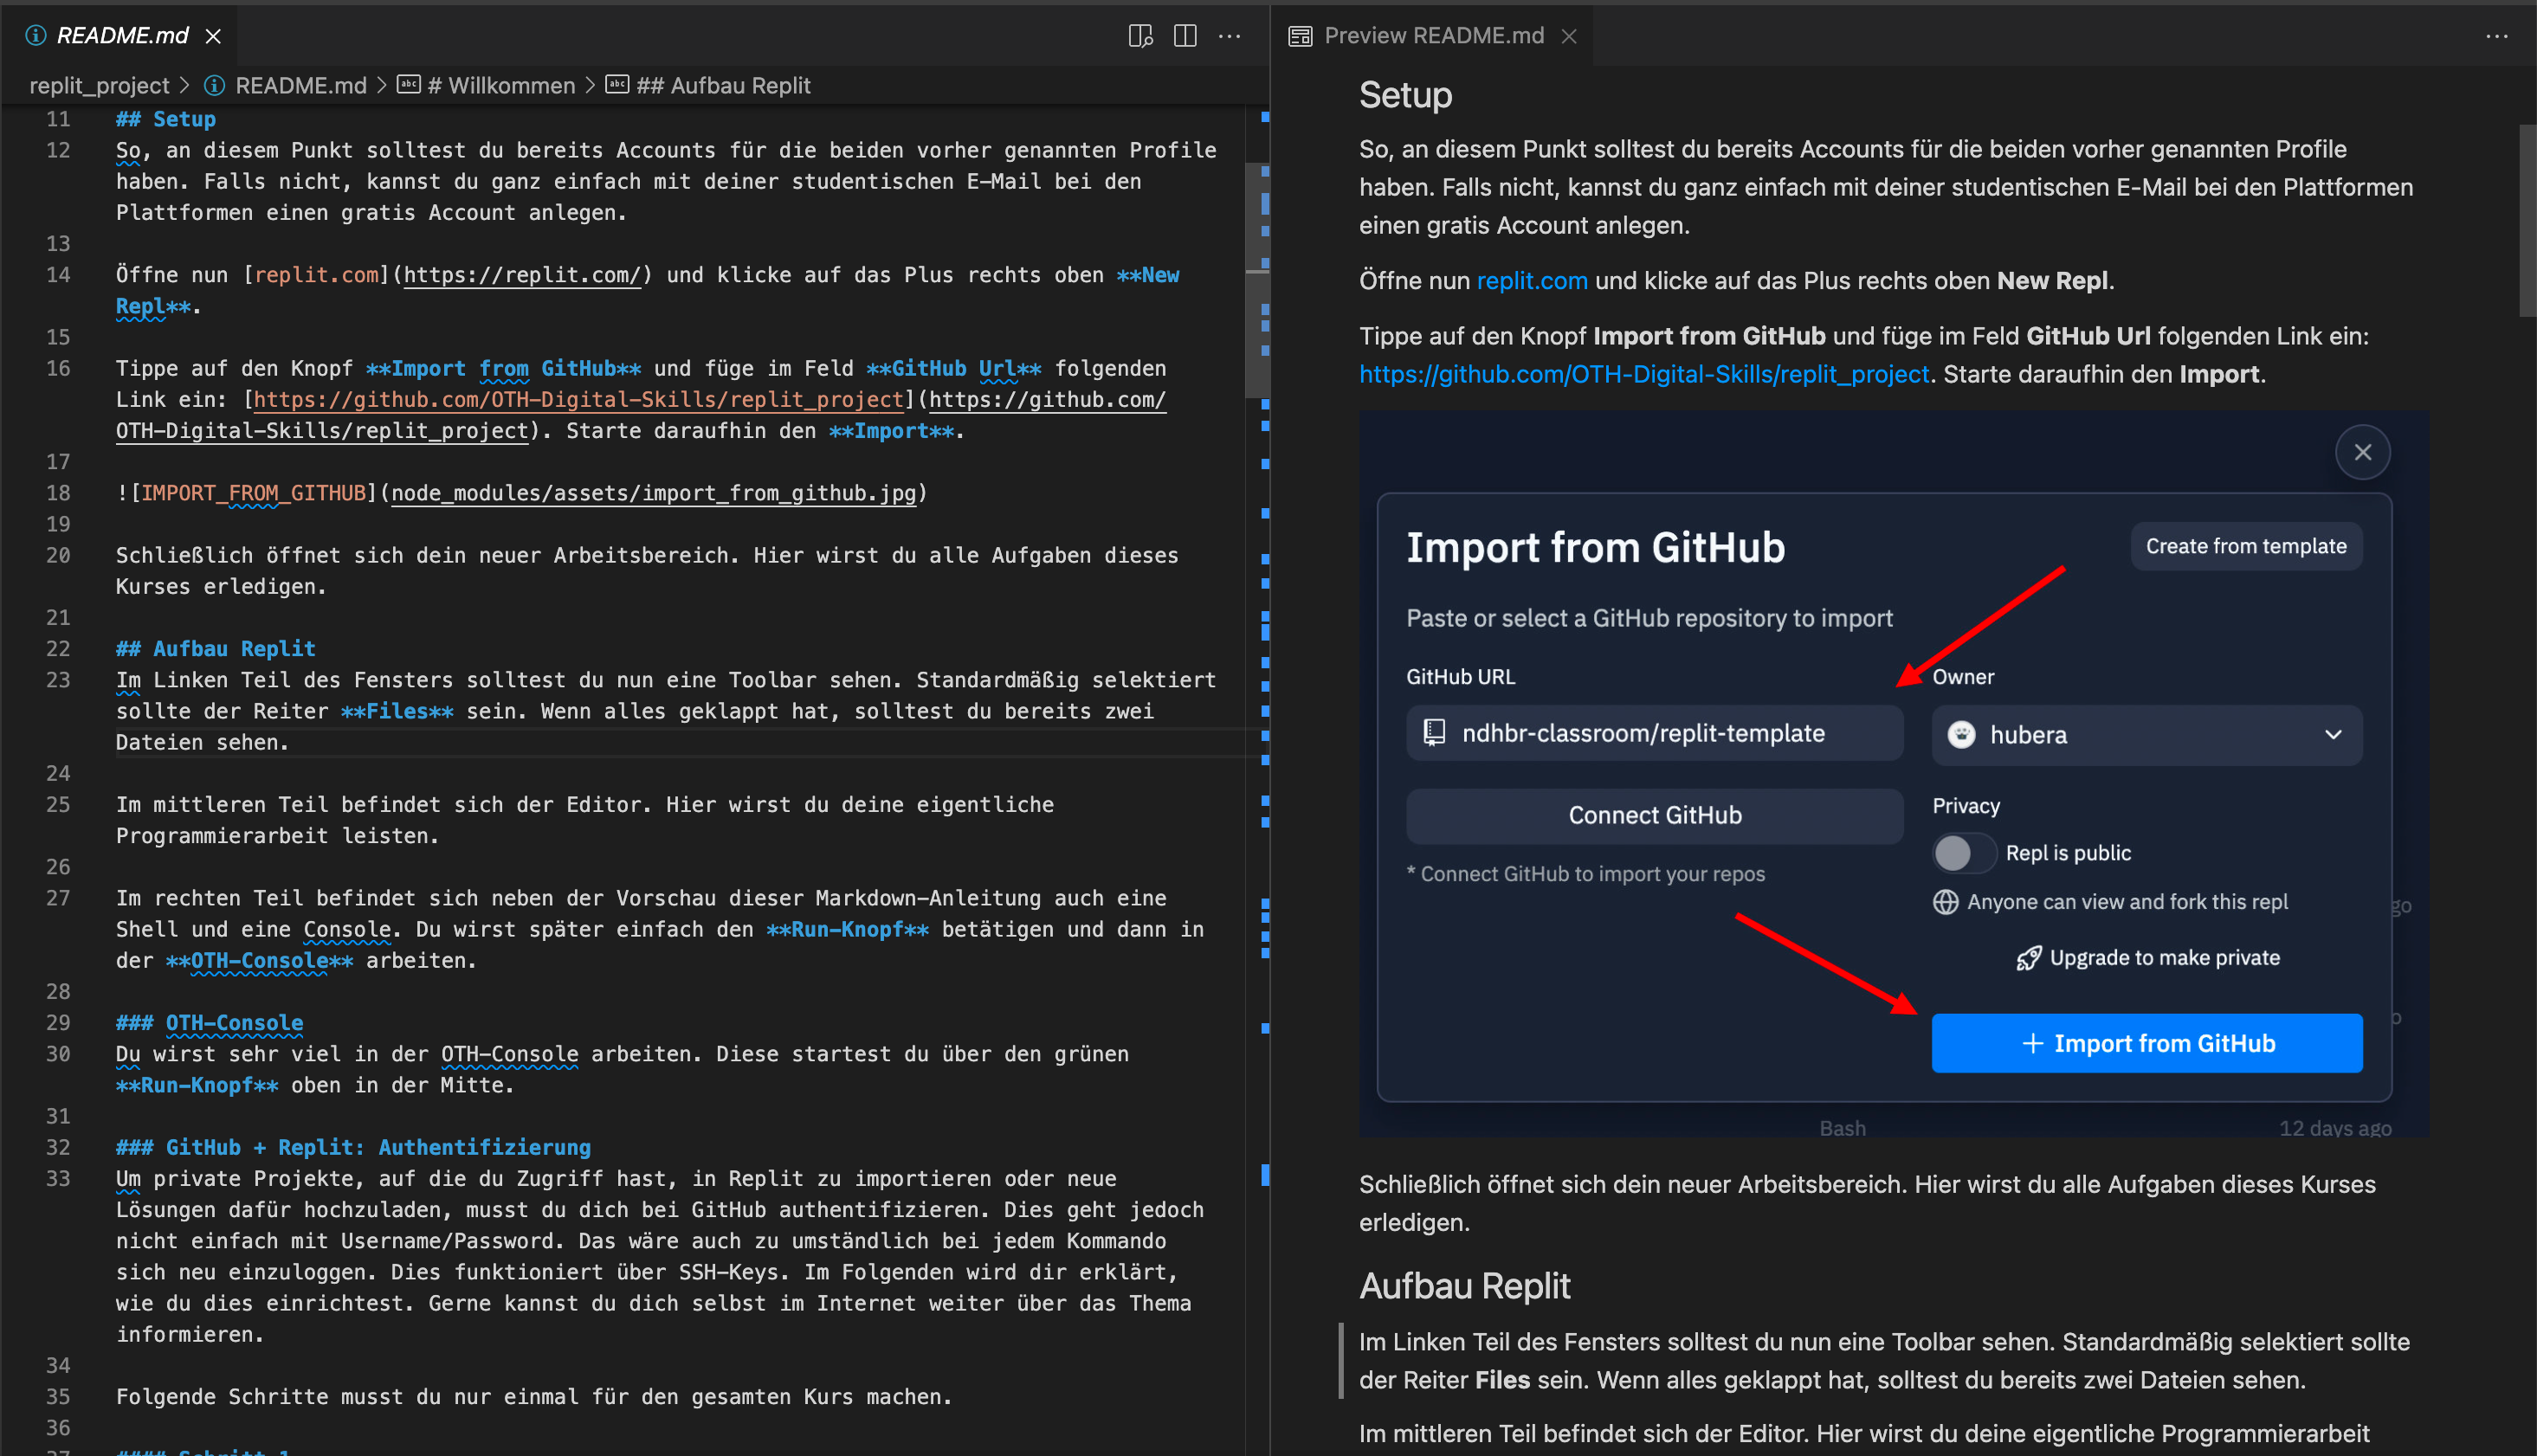
\includegraphics[width=\textwidth]{markdown}
    \caption{Erstellung eines Markdown-Dokuments}
    \bildquelle{Eigene Darstellung}
    \label{fig:markdown}
\end{figure}

\subsubsection{Replit als Online-Entwicklungsumgebung}
Der Programmierkurs soll für jeden Teilnehmer ohne komplizierte Installationen
durchführbar sein. Aus diesem Grund wurde die Entscheidung gefällt, eine
Online Entwicklungsumgebung einzusetzen.

Der Vorteil an Replit ist, dass man den Studierenden durch ein
Vorlagenrepository alle nötigen Konfigurationen und Programme im Vorhinein
bereitstellen kann. Sobald ein sogenanntes \emph{Repl} (Bezeichnung für
ein Projekt in Replit) mit der erwähnten Vorlage erstellt wurde, kann der
Studierende ohne Installation geräteübergreifend online programmieren
\parencite{replit-import-from-github}. Der Teilnehmer muss daraufhin lediglich
auf den \glqq Run\grqq{}-Knopf drücken, welcher die später näher erläuterte
\emph{OTH-Console} startet und schließlich alle benötigten Abhängigkeiten
bereitstellt.

\subsubsection{GitHub Classroom als Abgabe- und Bewertungssystem}
GitHub Classroom eignet sich, für den Einsatz an der Hochschule, vor allem durch
seine Flexibilität und Einfachheit. Durch diese Flexibilität ist es möglich,
GitHub Classroom nur als eine austauschbare Komponente des Systems zu sehen.
Classroom übernimmt im System die Rolle des Aufgabenservers. Hier werden alle
Aufgabenvorlagen, sowie alle Versuche der Studierenden gespeichert und bewertet.

Sollte diese Komponente des Systems ausfallen, besteht weiterhin Replit als
Online-IDE, sowie Tutors mit den jeweiligen Anleitungen. Dadurch muss lediglich
ein adäquater Ersatz für GitHub Classroom gefunden und installiert werden.